\documentclass[border=15pt]{standalone}
\usepackage{tikz}
\usetikzlibrary{arrows.meta, positioning, calc}
\usepackage{amsmath, amssymb}

\begin{document}

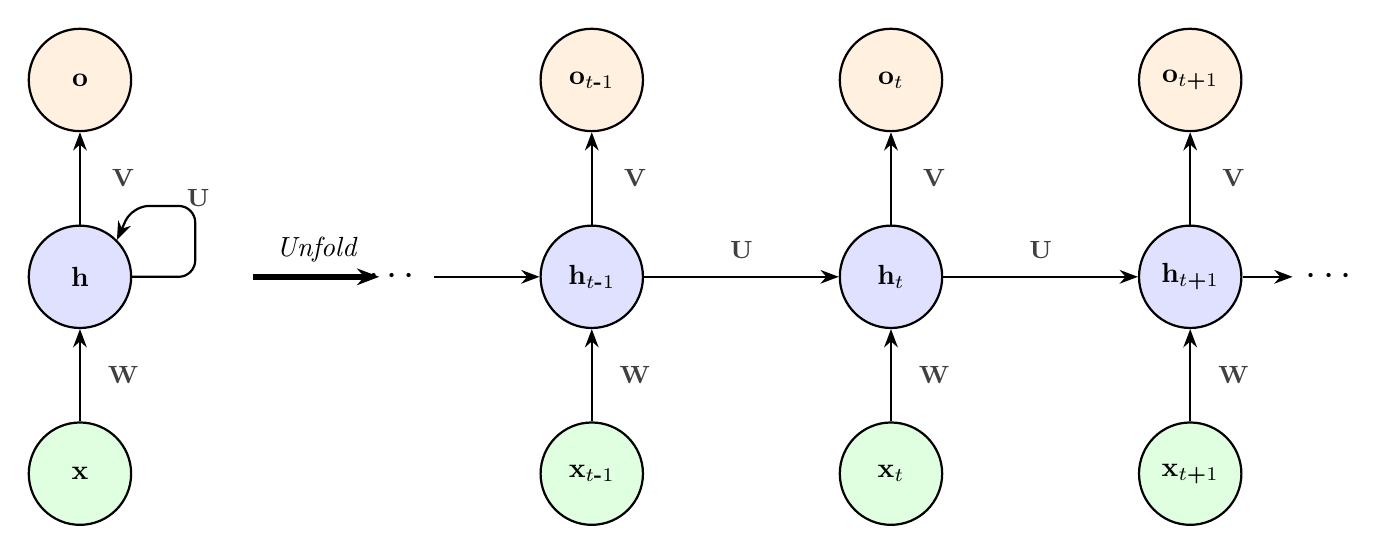
\begin{tikzpicture}[
    >=Stealth,
    rnnnode/.style={
        circle, draw, thick, minimum size=1.3cm, fill=blue!12,
        font=\normalsize\bfseries, inner sep=0pt
    },
    inputnode/.style={rnnnode, fill=green!12},
    outputnode/.style={rnnnode, fill=orange!12},
    arr/.style={draw, thick, ->},
    wlbl/.style={font=\small, text=gray!50!black},
]

% ================================================================
%  LEFT: FOLDED RNN CELL
% ================================================================
\node[rnnnode]    (h_fold) at (0, 2.5) {$\mathbf{h}$};
\node[inputnode]  (x_fold) at (0, 0)   {$\mathbf{x}$};
\node[outputnode] (o_fold) at (0, 5)   {$\mathbf{o}$};

% Self-loop: rounded rectangle path to the right of h
\draw[arr, rounded corners=6pt]
    (h_fold.east) -- ++(0.8, 0) -- ++(0, 0.9) -- ++(-0.8, 0) -- (h_fold.north east);
\node[wlbl] at (1.5, 3.5) {$\mathbf{U}$};

% Input -> Hidden (W label to the right, offset from arrow)
\draw[arr] (x_fold.north) -- (h_fold.south);
\node[wlbl] at (0.55, 1.25) {$\mathbf{W}$};

% Hidden -> Output (V label to the right, offset from arrow)
\draw[arr] (h_fold.north) -- (o_fold.south);
\node[wlbl] at (0.55, 3.75) {$\mathbf{V}$};

% ================================================================
%  UNFOLD ARROW
% ================================================================
\draw[-{Stealth[length=8pt, width=6pt]}, line width=2pt] (2.2, 2.5) -- (3.8, 2.5);
\node[font=\normalsize\itshape, above=2pt] at (3.0, 2.5) {Unfold};

% ================================================================
%  RIGHT: UNFOLDED RNN (t-1, t, t+1)
% ================================================================
\def\sep{3.8}
\def\xoff{6.5}

% --- t-1 ---
\node[rnnnode]    (h_tm1) at (\xoff, 2.5)       {$\mathbf{h}_{t\text{-}1}$};
\node[inputnode]  (x_tm1) at (\xoff, 0)          {$\mathbf{x}_{t\text{-}1}$};
\node[outputnode] (o_tm1) at (\xoff, 5)          {$\mathbf{o}_{t\text{-}1}$};

% --- t ---
\node[rnnnode]    (h_t) at (\xoff+\sep, 2.5)    {$\mathbf{h}_{t}$};
\node[inputnode]  (x_t) at (\xoff+\sep, 0)      {$\mathbf{x}_{t}$};
\node[outputnode] (o_t) at (\xoff+\sep, 5)      {$\mathbf{o}_{t}$};

% --- t+1 ---
\node[rnnnode]    (h_tp1) at (\xoff+2*\sep, 2.5) {$\mathbf{h}_{t\text{+}1}$};
\node[inputnode]  (x_tp1) at (\xoff+2*\sep, 0)   {$\mathbf{x}_{t\text{+}1}$};
\node[outputnode] (o_tp1) at (\xoff+2*\sep, 5)   {$\mathbf{o}_{t\text{+}1}$};

% --- W arrows (input -> hidden), labels to the right ---
\draw[arr] (x_tm1.north) -- (h_tm1.south);
\node[wlbl] at (\xoff+0.55, 1.25) {$\mathbf{W}$};

\draw[arr] (x_t.north) -- (h_t.south);
\node[wlbl] at (\xoff+\sep+0.55, 1.25) {$\mathbf{W}$};

\draw[arr] (x_tp1.north) -- (h_tp1.south);
\node[wlbl] at (\xoff+2*\sep+0.55, 1.25) {$\mathbf{W}$};

% --- V arrows (hidden -> output), labels to the right ---
\draw[arr] (h_tm1.north) -- (o_tm1.south);
\node[wlbl] at (\xoff+0.55, 3.75) {$\mathbf{V}$};

\draw[arr] (h_t.north) -- (o_t.south);
\node[wlbl] at (\xoff+\sep+0.55, 3.75) {$\mathbf{V}$};

\draw[arr] (h_tp1.north) -- (o_tp1.south);
\node[wlbl] at (\xoff+2*\sep+0.55, 3.75) {$\mathbf{V}$};

% --- U arrows (hidden -> hidden across time), labels above ---
\draw[arr] (h_tm1.east) -- (h_t.west);
\node[wlbl, above=3pt] at ($0.5*(h_tm1.east)+0.5*(h_t.west)$) {$\mathbf{U}$};

\draw[arr] (h_t.east) -- (h_tp1.west);
\node[wlbl, above=3pt] at ($0.5*(h_t.east)+0.5*(h_tp1.west)$) {$\mathbf{U}$};

% --- Left ellipsis for continuation ---
\node[font=\Large] at (\xoff - 2.5, 2.5) {$\cdots$};
\draw[arr] (\xoff - 2.0, 2.5) -- (h_tm1.west);

\node[font=\Large] at (\xoff + 2*\sep + 1.8, 2.5) {$\cdots$};
\draw[arr] (h_tp1.east) -- (\xoff + 2*\sep + 1.3, 2.5);

\end{tikzpicture}

\end{document}
